\chapter{Architektur  \label{chap_archtitektur}}
\todo{Auf jeden Fall noch in \cite{etsi302636-3} reinsehen}
\section{ITS Station Reference Architecture}
\todo{Evtl. kommt das in das Chapter Architektur}
Um das folgende Kapitel zu verstehen muss die \ac{ITS} Station Reference Architecture betrachtet werden. Eine Referenzarchitektur beschreibt ein allgemeines Modell einer Architektur. Das bedeutet, dass basierend auf dieser Architektur verschiedene Implementierungen existieren können. 

Die \ac{ITS} Station Reference Architecture unterscheidet sich grundlegend von bekannten Architekturen. Verglichen mit dem \ac{OSI} Modell kann man Gemeinsamkeiten erkennen:
\begin{itemize}
	\item Trennung der einzelnen Layer
	\item Definition von Service Primitiven zwischen den Layern
\end{itemize}

Bei der genaueren Beschreibung der Layer fällt auch auf, dass die Beschreibungen sich stellenweise auf das \ac{OSI} Modell beziehen. Der Hintergrund ist, dass die \ac{ITS} Station Reference Architecture an das \ac{OSI} Modell angelehnt ist. Es wurde aber um die Besonderheiten von \ac{ITS} erweitert.

Es gibt jedoch einen gravierenden Unterschied: In der \ac{ITS} Station Reference Architecture sind Cross Layer vorgesehen. Das \ac{OSI} Referenzmodell ist wasserfallartig aufgebaut. Das bedeutet, dass die einzelnen Layer übereinander angeordnet sind. Jeder Layer hat jeweils nur zu dem direkt über- und unterliegenden Layer eine Schnittstelle. Cross Layer sind Layer, die in mehrere dieser Schichten Schnittstellen haben. Im Fall der \ac{ITS} Station Reference Architecture sind das die Layer \glqq Management\grqq~ und \glqq Security\grqq. Sie haben Schnittstellen, bzw. Primitiven in alle anderen Layer. 

Möglichkeit Aufgaben dieser Layer sind:
\subsection{Management Layer}
Beschrieben in \cite{etsi1027232}
\todo{Management Layer genauer beschreiben}

\subsection{Security Layer}

\subsection{Access}
Der Access Layer entspricht den \ac{OSI} Layern 1 und 2. 

\subsection{Networking \& Transporting}
Der Networking \& Transporting Layer entspricht den \ac{OSI} Layern 3 und 4.

\subsection{Facilities}
Der Facilities Layer entspricht den \ac{OSI} Layern 5, 6 und 7

\subsection{Applications}


\begin{figure}
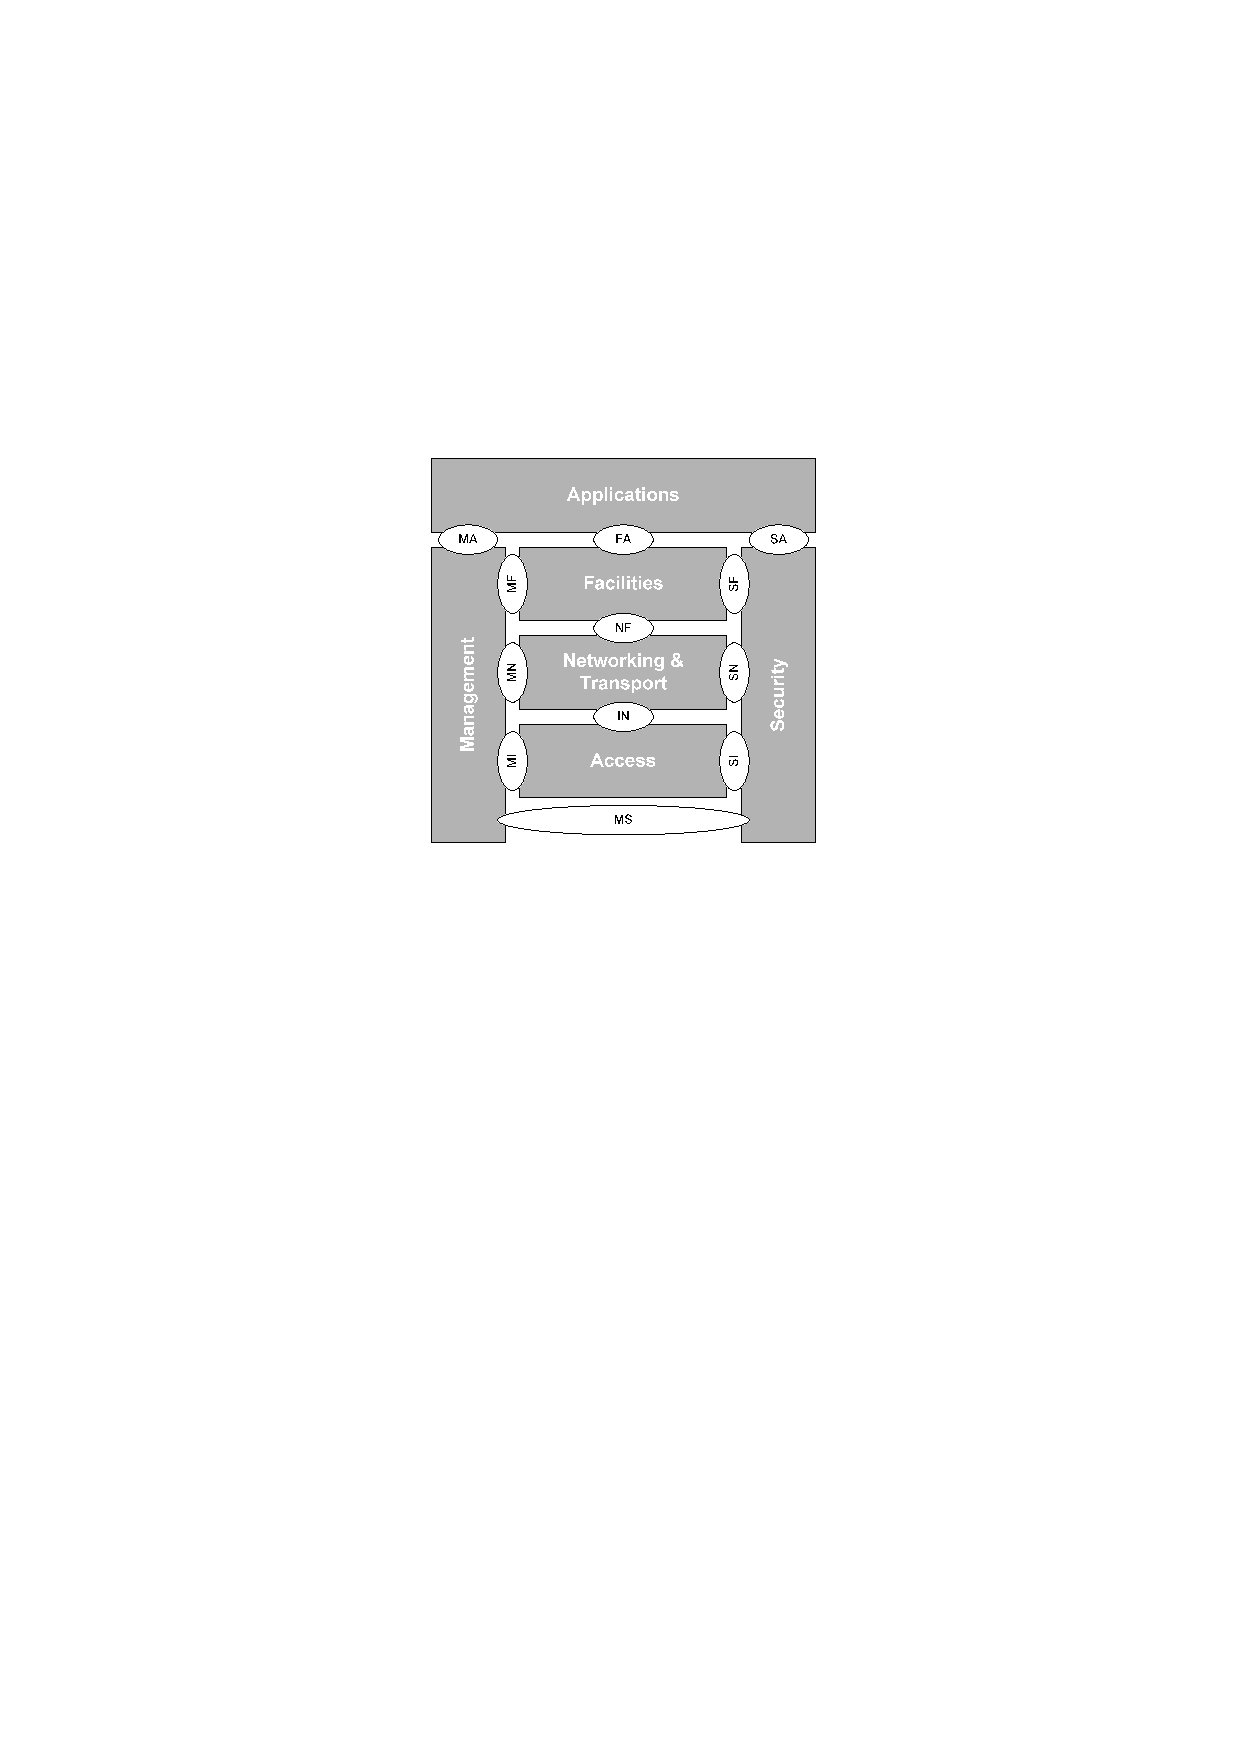
\includegraphics[width=0.75\textwidth]{content/images/02_architektur/stationReferenceArchitecture.pdf}
\caption{Darstellung der ITS Station Reference Architecture \cite{etsi2010302}}
\label{fig:funktionsweise_referenceArchitecture}
\end{figure}

\section{Cross Layer}

\section{Data Security}

